\setcounter{step}{0}
%------------------------------------------
% information doc
\subsection{Dhal}
%------------------------------------------

\begin{ingredient}

%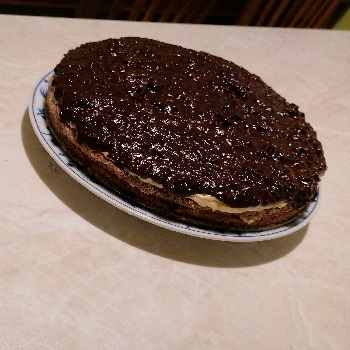
\includegraphics[height=5.5cm]{images/daim}
\def\portions{4}%
\textbf{{\normalsize Ingrediencie (\portions porcie):}}

%\vspace{0.5cm}
\begin{main}
	\item 1ks cibuľa
	\item 2 strúčiky cesnak
	\item 10g čerstvý zázvor 
	\item 3ks nakrájané paradajky
	\item 300-400ml kokosové mlieko
	\item 200g červená šošovica
\end{main}
\begin{subingredient}{korenie}
	\item 1 PL kari
	\item 1 PL mletá rasca
	\item bobkový list
	\item chilli paprička
	\item 1/2 KL mletý koriander
\end{subingredient}

\end{ingredient}
\begin{recipe}
\textbf{{\normalsize Príprava:}}
\begin{enumerate}
\item{Na oleji do sklovita posmažíme nakrájanú cibuľku}
\item{Pridám nadrobno nakrájaný zázvor, pretlačený cesnak, korenie. Smažíme 1-2 minúty.}
\item{Pridáme nakrájané paradajky, kokosové mlieko, vodu, červenú šošovicu.}
\item{Varíme kým šošovica nezmäkne. Ak je to príliš husté, pridáme vodu.}
\item{Pridáme soľ podľa chuti}
\end{enumerate}

\end{recipe}

\begin{notes}

\end{notes}	
\clearpage